\documentclass{beamer}
\usetheme{Madrid}
\usepackage{pifont}
\usepackage{amsmath}
\usepackage{geometry} 
\usepackage{svg}
\usepackage{graphicx}
\usepackage{tikz}
\usetikzlibrary{shapes.geometric, arrows, positioning}

\usetheme{Madrid}
\usecolortheme{default}



% ==========================================
% COMPACT TIKZ STYLES
% ==========================================
% 1. Reduced minimum width/height
% 2. Added font=\small or \footnotesize
% 3. Added 'aspect=2' to decision to make diamond flatter/wider
% ==========================================
\usepackage{listings}
\definecolor{codegreen}{rgb}{0,0.6,0}
\lstset{
	language=Python,
	basicstyle=\ttfamily\tiny,
	breaklines=true,
	xleftmargin=0pt,
	framexleftmargin=0pt,
	showstringspaces=false
}
\tikzset{
	process/.style={
		rectangle, 
		rounded corners, 
		minimum width=2.2cm, 
		minimum height=0.8cm, 
		text centered, 
		draw=black, 
		fill=blue!30,
		font=\small
	},
	data/.style={
		rectangle, 
		minimum width=2.2cm, 
		minimum height=0.8cm, 
		text centered, 
		draw=black, 
		fill=green!30,
		font=\small
	},
	decision/.style={
		diamond, 
		aspect=2.5, 
		minimum width=2.5cm, 
		minimum height=0.8cm, 
		text centered, 
		draw=black, 
		fill=orange!30,
		font=\footnotesize,
		inner sep=1pt
	},
	arrow/.style={thick,->,>=stealth}
}

\graphicspath{ {./assets/} }
\usetikzlibrary{positioning}



\title{Adaptasi Positional Encoding pada Arsitektur Transformer untuk Sintesis Notasi Gamelan yang Koheren dan Terkendali}
\author{Arif Akbarul Huda}

\begin{document}
	\begin{frame}
		\titlepage
	\end{frame}
	
	\begin{frame}
		\frametitle{Previous Work}
		\framesubtitle{Decoding PDF files}
		
		% 1. TOP ROW: TWO COLUMNS (50% each)
		\begin{columns}
			% --- Left Column (Row 1, Col 1) ---
			\begin{column}{0.48\textwidth}
				\centering
				\includegraphics[width=0.9\linewidth]{notasi-ayak-nem-slendro.png}
				\footnotesize{Notasi gamelan Ayak-ayakan Nem Slendro pt. Nem}
			\end{column}
			
			% --- Right Column (Row 1, Col 2) ---
			\begin{column}{0.48\textwidth}
				\centering
				\includegraphics[width=0.9\linewidth]{cmap-font-balungan.png}
				\footnotesize{Cmap font balungan.}
			\end{column}
		\end{columns}
		
		% Optional: Add a small vertical space between the rows
		\vspace{0.5em}
		\hrule % Optional: A horizontal line to visually separate the rows
		
		% 2. BOTTOM ROW: ONE MERGED COLUMN
		% We use \vfill to push the content to the bottom and a minipage to control its width
		\vfill 
		\begin{minipage}{\textwidth} % Minipage spans the full text width
			\centering
			
			\begin{figure}
				\centering
				\includegraphics[width=0.75 \linewidth]{notasi-ayak-nem-slendro-decoded.png}
				\caption{Notasi ayakan decoded}			
			\end{figure}
		\end{minipage}
		
	\end{frame}
	
	\begin{frame}
		\frametitle{Previous Work}
		\framesubtitle{Plotting Structure}
		\begin{columns}
			
			% --- First Column (Left Image) srepeg-tlutur-sl-sanga.png---
			\begin{column}{0.5\textwidth}
				\begin{figure}
					\centering
					\includegraphics[width=1 \linewidth]{srepeg-tlutur-sl-sanga.png}
					\caption{Notasi Gamelan}			
				\end{figure}		
			\end{column}
			
			% --- Second Column (Right Image) ---
			\begin{column}{0.5\textwidth}
				\begin{figure}
					\centering
					\includegraphics[width=1 \linewidth]{plot-struktur-gamelan.png}
					\caption{Plot Struktur}			
				\end{figure}		
			\end{column}
		\end{columns}
	\end{frame}
	% ============================================
	% PART 1: Dataset
	% ============================================
	\begin{frame}
		\frametitle{Dataset Insight}
		\begin{columns}
			
			\begin{column}{0.5 \textwidth}
				\begin{figure}
					\centering
					\includegraphics[width=1 \linewidth]{top_cited.png}
				\end{figure}
			\end{column}
			
			\begin{column}{0.5 \textwidth}
				Dataset Overview
				\begin{itemize}
					\item  Total Songs : 189
					\item  Laras : 2
					\item  Cited in Research : 100\%
				\end{itemize}
				
			\end{column}
		\end{columns}
	\end{frame}
	% ============================================
	% PART 1: Dataset
	% ============================================
	\begin{frame}{Dataset Insight}
		\begin{center}
			\includegraphics[height=0.8\textheight]{distribution_dataset.png}
		\end{center}
	\end{frame}
	% ============================================
	% PART 1: Dataset
	% ============================================
	\begin{frame}{Dataset Insight}
		\begin{center}
			\includegraphics[width=0.8\textwidth]{pathet_distribution.png}
		\end{center}
	\end{frame}
	% ============================================
	% PART 1: Dataset
	% ============================================
	\begin{frame}{Dataset Insight}
	\begin{center}
		\includegraphics[width=0.8\textwidth]{structure_distribution.png}
	\end{center}
	\end{frame}
	% ============================================
	% PART 1: Dataset
	% ============================================
	\begin{frame}{Dataset Insight}
		\begin{center}
			\includegraphics[width=0.8\textwidth]{notation_distribution.png}
		\end{center}
	\end{frame}
	% ============================================
	% PART 1: Dataset
	% ============================================
	\begin{frame}{Dataset Insight}
		\begin{center}
			\includegraphics[width=0.8\textwidth]{notation_heatmap.png}
		\end{center}
	\end{frame}
	% ============================================
	% SLIDE 1: Overview (Compact)
	% ============================================
	\begin{frame}{System Overview}
		\begin{center}
			% Reduced node distance to match smaller nodes
			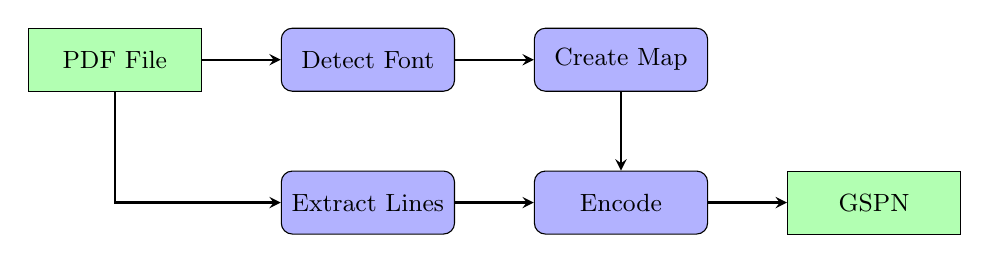
\begin{tikzpicture}[node distance=1.5cm]
				\node (pdf) [data] {PDF File};
				\node (font) [process, right=1cm of pdf] {Detect Font};
				\node (map) [process, right=1cm of font] {Create Map};
				\node (extract) [process, below=1cm of font] {Extract Lines};
				\node (encode) [process, right=1cm of extract] {Encode};
				\node (output) [data, right=1cm of encode] {GSPN};
				
				\draw [arrow] (pdf) -- (font);
				\draw [arrow] (font) -- (map);
				\draw [arrow] (pdf) |- (extract);
				\draw [arrow] (map) -- (encode); % Changed path for clearer flow
				\draw [arrow] (extract) -- (encode);
				\draw [arrow] (encode) -- (output);
			\end{tikzpicture}
		\end{center}
	\end{frame}

	% ============================================
	% SLIDE 2: Font Detection
	% ============================================
	\begin{frame}{Step 1: Font Detection}
		\begin{center}
			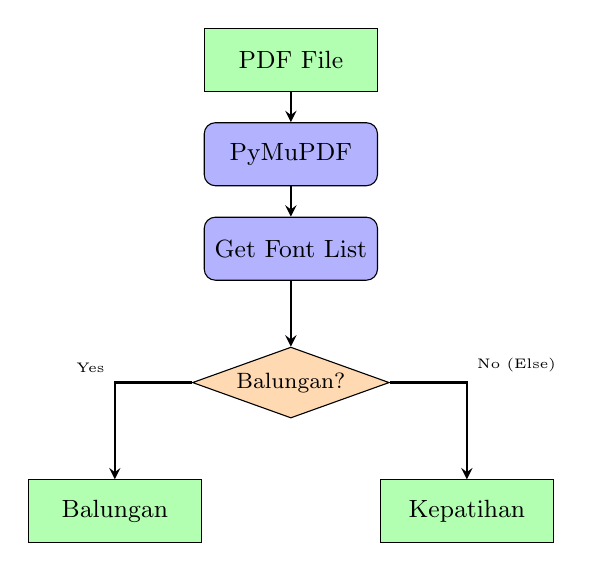
\begin{tikzpicture}[node distance=1.2cm]
				\node (start) [data] {PDF File};
				\node (open) [process, below of=start] {PyMuPDF};
				\node (getfonts) [process, below of=open] {Get Font List};
				\node (detect) [decision, below of=getfonts, yshift=-0.5cm] {Balungan?};
				
				% Branches
				\node (balungan) [data, below left=1cm and 0.5cm of detect] {Balungan};
				\node (kepatihan) [data, below right=1cm and 0.5cm of detect] {Kepatihan};
				
				\draw [arrow] (start) -- (open);
				\draw [arrow] (open) -- (getfonts);
				\draw [arrow] (getfonts) -- (detect);
				\draw [arrow] (detect) -| node[anchor=south east, font=\tiny] {Yes} (balungan);
				\draw [arrow] (detect) -| node[anchor=south west, font=\tiny] {No (Else)} (kepatihan);
			\end{tikzpicture}
		\end{center}
	\end{frame}

	% ============================================
	% SLIDE 3: Glyph Map Creation
	% ============================================
	\begin{frame}{Step 2: Glyph Map Creation}
		\begin{center}
			% Horizontal layout allows smaller nodes to fit better on one line
			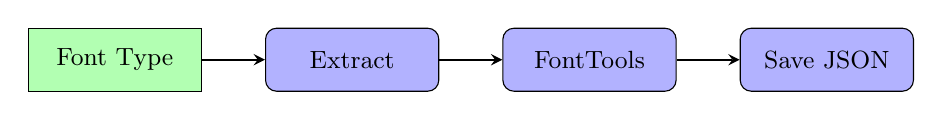
\begin{tikzpicture}[node distance=1.2cm]
				\node (fonttype) [data] {Font Type};
				\node (extract) [process, right=0.8cm of fonttype] {Extract};
				\node (tools) [process, right=0.8cm of extract] {FontTools};
				\node (json) [process, right=0.8cm of tools] {Save JSON};
				
				\draw [arrow] (fonttype) -- (extract);
				\draw [arrow] (extract) -- (tools);
				\draw [arrow] (tools) -- (json);
			\end{tikzpicture}
			
			\vspace{1cm}
			
			\textbf{Example Output (JSON):}
			\begin{columns}
				\column{0.4\textwidth}
				\begin{block}{Balungan}
					\scriptsize \texttt{"H": "1", "I": "2"}
				\end{block}
				\column{0.4\textwidth}
				\begin{block}{Kepatihan}
					\scriptsize \texttt{"1": "1", "e": "3a"}
				\end{block}
			\end{columns}
			
		\end{center}
	\end{frame}
	% ============================================
	% SLIDE 4: Line Extraction
	% ============================================
	\begin{frame}{Step 3: Line Extraction}
		\begin{center}
			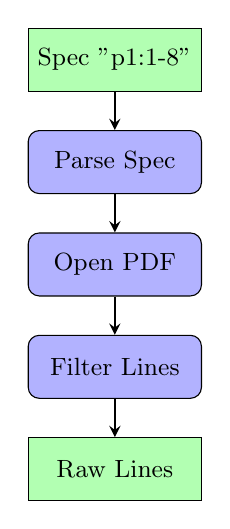
\begin{tikzpicture}[node distance=1.3cm]
				\node (spec) [data] {Spec "p1:1-8"};
				\node (parse) [process, below of=spec] {Parse Spec};
				\node (open) [process, below of=parse] {Open PDF};
				\node (filter) [process, below of=open] {Filter Lines};
				\node (out) [data, below of=filter] {Raw Lines};
				
				\draw [arrow] (spec) -- (parse);
				\draw [arrow] (parse) -- (open);
				\draw [arrow] (open) -- (filter);
				\draw [arrow] (filter) -- (out);
			\end{tikzpicture}
		\end{center}
	\end{frame}
	
	% ============================================
	% SLIDE 5: Encoding Logic
	% ============================================
	\begin{frame}{Step 4: Encoding Logic}
		\begin{center}
			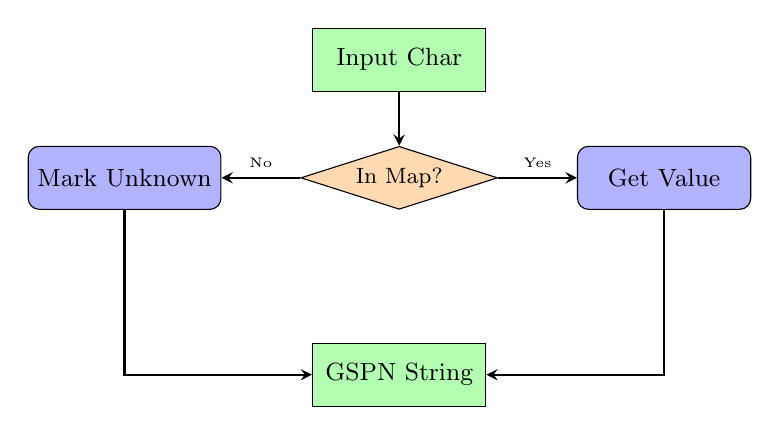
\begin{tikzpicture}[node distance=1.5cm]
				\node (input) [data] {Input Char};
				\node (check) [decision, below of=input] {In Map?};
				\node (map) [process, right=1cm of check] {Get Value};
				\node (unknown) [process, left=1cm of check] {Mark Unknown};
				\node (out) [data, below of=check, yshift=-1cm] {GSPN String};
				
				\draw [arrow] (input) -- (check);
				\draw [arrow] (check) -- node[above, font=\tiny] {Yes} (map);
				\draw [arrow] (check) -- node[above, font=\tiny] {No} (unknown);
				\draw [arrow] (map) |- (out);
				\draw [arrow] (unknown) |- (out);
			\end{tikzpicture}
		\end{center}
	\end{frame}
	
	% ============================================
	% SLIDE 6: Complete Flow (Top-Down)
	% ============================================
	\begin{frame}{Complete Processing Flow}
		\begin{center}
			% Scaling the whole picture down slightly to ensure fit
			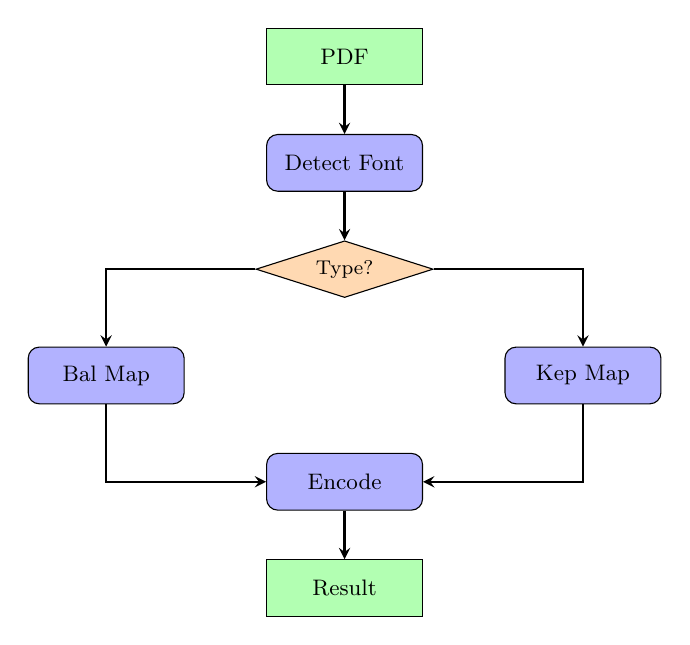
\begin{tikzpicture}[scale=0.9, transform shape, node distance=1.5cm]
				\node (pdf) [data] {PDF};
				\node (detect) [process, below of=pdf] {Detect Font};
				\node (choice) [decision, below of=detect] {Type?};
				
				\node (bmap) [process, left=1cm of choice, yshift=-1.5cm] {Bal Map};
				\node (kmap) [process, right=1cm of choice, yshift=-1.5cm] {Kep Map};
				
				\node (encode) [process, below of=choice, yshift=-1.5cm] {Encode};
				\node (result) [data, below of=encode] {Result};
				
				\draw [arrow] (pdf) -- (detect);
				\draw [arrow] (detect) -- (choice);
				\draw [arrow] (choice) -| (bmap);
				\draw [arrow] (choice) -| (kmap);
				\draw [arrow] (bmap) |- (encode);
				\draw [arrow] (kmap) |- (encode);
				\draw [arrow] (encode) -- (result);
			\end{tikzpicture}
		\end{center}
	\end{frame}

	% Slide 1: Compact Overview
	\begin{frame}[fragile]{Abiyasa: Gamelan Digitalization}
		\begin{columns}[c]
			\begin{column}{0.40\textwidth}
				\textbf{Capabilities}
				\begin{itemize}
					\item \textbf{Extraction}: PDF to data.
					\item \textbf{Systems}: Balungan \& Kepatihan.
					\item \textbf{Encoders}: GSPN/QAP.
				\end{itemize}
				\textbf{Install}
				\begin{lstlisting}[language=bash]
pip install abiyasa
				\end{lstlisting}
			\end{column}
			
			\begin{column}{0.58\textwidth}
				\begin{exampleblock}{Quick Start API}
					\begin{lstlisting}[language=python]
import abiyasa
						
# Load and encode 5 items
data = abiyasa.load_data(
	encoder='GSPN', 
	notation_system='kepatihan', 
	limit=5
)
						
for item in data:
	print(item['encoded_data'][0]['encoded'])
					\end{lstlisting}
				\end{exampleblock}
			\end{column}
		\end{columns}
		
		\begin{block}{Dataset Format}
			Curated JSON including titles, PDF sources, and line-specific markers (\texttt{p1:1-5}).
		\end{block}
	\end{frame}
	
	% Slide 2: Technical Logic
	\begin{frame}{The GSPN Encoding Strategy}
		The \textbf{Gendhing Scientific Pitch Notation (GSPN)} is the core computational format.
		
		\begin{alertblock}{Formula: $T + W + V + G$}
			\begin{itemize}
				\item \textbf{T (Note)}: 0--7 (0 = rest).
				\item \textbf{W (Octave)}: empty (mid), a (low), b (high).
				\item \textbf{V (Value)}: empty (1), A (1/2), B (1/4).
				\item \textbf{G (Legato)}: x (start), y (end).
			\end{itemize}
		\end{alertblock}
		
		\begin{table}[]
			\tiny
			\centering
			\begin{tabular}{|l|l|l|}
				\hline
				\textbf{System} & \textbf{Notation Example} & \textbf{GSPN Result} \\ \hline
				Balungan & \texttt{F F} & \texttt{6a 6a} \\ \hline
				Balungan & \texttt{-\_ \_F\_} & \texttt{0A 6aA} \\ \hline
				Kepatihan & \texttt{e t y u} & \texttt{3a 5a 6a 7a} \\ \hline
				Kepatihan & \texttt{1 2 3} & \texttt{1 2 3} \\ \hline
			\end{tabular}
		\end{table}
	\vfill
	\centering
	\scriptsize \textit{Based on research by Syarif et al. (2020)}
	\end{frame}

	\begin{frame}
		\frametitle{Insight}
		\framesubtitle{Chapter 4. Music Structure Analysis}
		\begin{columns}
			
			% --- First Column (Left Image) srepeg-tlutur-sl-sanga.png--- structural-analysis.png
			\begin{column}{0.5 \textwidth}
				\begin{figure}
					\centering
					\includegraphics[width=1 \linewidth]{structural-analysis.png}
					\caption{4.1. From the book}
				\end{figure}
			\end{column}
			
			% --- Second Column (Right Image) ---
			\begin{column}{0.5 \textwidth}
				The General Goal of Music Structural Analysis
				\begin{itemize}
					\item  Temporal Segmentation
					\item  Structural Identification
					\item  Categorical Grouping
				\end{itemize}
				The methods
				\begin{itemize}
					\item  Repition-based
					\item  Novelty-based
					\item  Homogeneity-based
				\end{itemize}
				
			\end{column}
		\end{columns}
	\end{frame}
	\begin{frame}
		\frametitle{Insight}
		\framesubtitle{Chapter 4. Music Structure Analysis}
		\begin{columns}
			
			% --- First Column (Left Image) srepeg-tlutur-sl-sanga.png--- structural-analysis.png
			\begin{column}{0.5 \textwidth}
				\begin{figure}
					\centering
					\includegraphics[width=1 \linewidth]{structure-annotatoins-labeling-evaluation.png}
					\caption{4.30. From the book}
				\end{figure}
			\end{column}
			
			% --- Second Column (Right Image) ---
			\begin{column}{0.5 \textwidth}
				Evaluation
				\begin{itemize}
					\item  Precision, Recall, F-Measure
					\item  Structure Annotations
					\item  Labeling Eval.
					\item  Boundary Eval.
					\item  Thumbnail Eval.
				\end{itemize}
				
			\end{column}
		\end{columns}
	\end{frame}
	\begin{frame}
		\frametitle{Insight}
		
		
		Subjective evaluation are
		\begin{itemize}
			\item  Unscalable
			\item  Inability to Guide Improvement
			\item  Missing the "Why"
		\end{itemize}
	 	\vspace{1cm}
		\tiny de Berardinis, J., Cangelosi, A. and Coutinho, E. (2022) “Measuring the Structural Complexity of Music: From Structural Segmentations to the Automatic Evaluation of Models for Music Generation,” IEEE/ACM Transactions on Audio, Speech, and Language Processing, 30, pp. 1963–1976. Available at: https://doi.org/10.1109/TASLP.2022.3178203.
	\end{frame}

	
	
	\begin{frame}
		\frametitle{Insight}
		\tiny Kader FB, Karmaker S. A Survey on Evaluation Metrics for Music Generation [Internet]. arXiv; 2025 [cited 2025 Nov 19]. Available from: http://arxiv.org/abs/2509.00051
	
		\begin{figure}
			\centering
			\includegraphics[width=1 \linewidth]{taxonomy-evaluation-symbolic-music-generation}
			\caption{Cuplikan taxonomy evaluasi}			
		\end{figure}
	\end{frame}

	
	\begin{frame}
		\frametitle{P.O.C}
		\begin{itemize}
			\item Experimental evaluasi struktur pada dataset
			\item Experimental evaluasi struktur pada previous paper
		\end{itemize}
	\end{frame}
	
\end{document}
